\documentclass[12pt, twoside]{article}
\input{/Users/chris/github/course-files/docs/ib/preamble}

\fancyhead[LO]{La Scuola d'Italia / Dr.\ Huson / IB Math 12 HL \\* 17 November 2026}
\fancyhead[RO]{\fbox{\begin{minipage}{6cm}\footnotesize Nickname:\\[0.5cm]\end{minipage}}}
\fancyfoot[C]{\thepage}

\begin{document}
\subsubsection*{3.6 Quiz: Periodic Functions (HL)}

Problems 1--3: \textbf{no calculator}. Problems 4--6: a calculator is
allowed. Use the answer boxes for Problems 1--4; answer Problems 5 and 6 on
lined paper; if a box runs out, continue on lined paper and label the
problem and part. Give answers exactly, or correct to three significant
figures.

\begin{enumerate}[itemsep=0.15cm]

%--- Problem 1: Graph of f(x) = acos(bx) + d with a < 0: a, d, b from min (0, -5) and max (pi/3, 3); rewrite as p sin(3(x - q)) - 1; dashed g = f(x + pi/4): expression and exact g(0) [10 marks] ---
%--- Source: Original (AA HL 2.11, 3.7, 3.5); modelled on AA_HL_2025_Nov_P2_TZ1 Q4 and AA_HL_2021_Nov_P2 Q9(g) ---
\item[1.] [Maximum mark: 10] \hfill \textbf{No calculator}

The solid curve is the graph of $y = f(x)$, where $f(x) = a\cos(bx) + d$,
for $0 \le x \le \pi$, with $a \in \mathbb{R}$ and $b > 0$. It has a minimum
point at $(0,\ -5)$ and a maximum point at
$\left(\frac{\pi}{3},\ 3\right)$. The dashed curve is the graph of
$y = g(x)$: the graph of $f$ translated horizontally by $\frac{\pi}{4}$.

\begin{center}
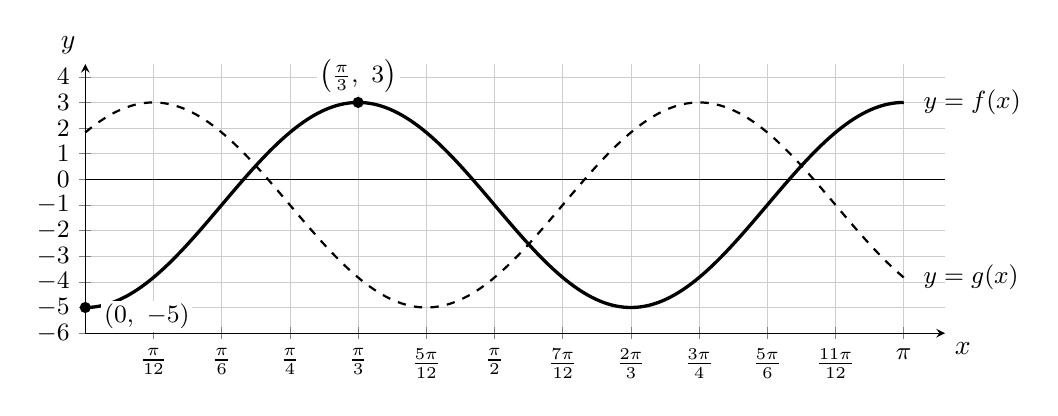
\begin{tikzpicture}
\begin{axis}[
  axis lines=left,
  xlabel={$x$}, ylabel={$y$},
  xlabel style={at={(axis description cs:1,0)}, anchor=north west},
  ylabel style={at={(axis description cs:0,1)}, anchor=south east, rotate=-90},
  xmin=0, xmax=3.3, ymin=-6, ymax=4.5,
  xtick={0.2618,0.5236,0.7854,1.0472,1.3090,1.5708,1.8326,2.0944,2.3562,2.6180,2.8798,3.1416},
  xticklabels={$\frac{\pi}{12}$,$\frac{\pi}{6}$,$\frac{\pi}{4}$,$\frac{\pi}{3}$,$\frac{5\pi}{12}$,$\frac{\pi}{2}$,
    $\frac{7\pi}{12}$,$\frac{2\pi}{3}$,$\frac{3\pi}{4}$,$\frac{5\pi}{6}$,$\frac{11\pi}{12}$,$\pi$},
  ytick={-6,-5,...,4},
  grid=major, grid style={line width=0.2pt, gray!40},
  tick label style={font=\small},
  width=12.5cm, height=5.0cm, clip=false,
]
  \draw[thin] (axis cs:0,0) -- (axis cs:3.3,0);
  \addplot[very thick, domain=0:3.1416, samples=200] {-4*cos(deg(3*x)) - 1};
  \addplot[thick, dashed, domain=0:3.1416, samples=200] {-4*cos(deg(3*x + 2.3562)) - 1};
  \addplot[only marks, mark=*, mark size=1.8pt] coordinates {(0,-5) (1.0472,3)};
  \node[anchor=west, fill=white, inner sep=1pt, font=\small] at (axis cs:0.06,-5.35) {$(0,\ -5)$};
  \node[anchor=south, fill=white, inner sep=1pt, font=\small] at (axis cs:1.0472,3.25) {$\left(\frac{\pi}{3},\ 3\right)$};
  \node[anchor=west, font=\small] at (axis cs:3.18,3) {$y = f(x)$};
  \node[anchor=west, font=\small] at (axis cs:3.18,-3.83) {$y = g(x)$};
\end{axis}
\end{tikzpicture}
\end{center}

\begin{enumerate}[itemsep=0.1cm]
  \item Find the value of $a$ and the value of $d$. \hfill [2]
  \item Find the value of $b$. \hfill [2]
  \item $f(x)$ can also be written as $f(x) = p\sin\bigl(b(x - q)\bigr) - 1$,
  where $p > 0$. Write down the value of $p$, and find the smallest positive
  value of $q$. \hfill [3]
  \item
  \begin{enumerate}[label=(\roman*), itemsep=0.05cm]
    \item Write down an expression for $g(x)$. \hfill [1]
    \item Find the exact value of $g(0)$. \hfill [2]
  \end{enumerate}
\end{enumerate}

\begin{tikzpicture}
  \draw (-0.6,0) rectangle (14.6,5.8);
  \foreach \y in {1,2,...,5} \draw[dotted] (0,\y)--(14.1,\y);
\end{tikzpicture}

\newpage

%--- Problem 2: sec(theta) = -4 in quadrant III: tan and cosec exactly; cos 105 deg by compound angle; 105 deg in radians, sec(7pi/12) with rational denominator [10 marks] ---
%--- Source: Original (AA HL 3.4, 3.6, 3.9, 3.10); modelled on AA_HL_2021_May_P1_TZ1 Q6 (cosec/cot) ---
\item[2.] [Maximum mark: 10] \hfill \textbf{No calculator}

It is given that $\sec\theta = -4$, where $\pi < \theta < \dfrac{3\pi}{2}$.

\begin{enumerate}[itemsep=0.1cm]
  \item Find the exact value of $\tan\theta$. \hfill [3]
  \item Find the exact value of $\operatorname{cosec}\theta$. \hfill [2]
  \item By writing $105^\circ = 60^\circ + 45^\circ$, find the exact value of
  $\cos 105^\circ$. \hfill [2]
  \item Write $105^\circ$ in radians. Hence find the exact value of
  $\sec\dfrac{7\pi}{12}$, giving your answer with a rational denominator.
  \hfill [3]
\end{enumerate}

\begin{tikzpicture}
  \draw (-0.6,0) rectangle (14.6,15.3);
  \foreach \y in {1,2,...,14} \draw[dotted] (0,\y)--(14.1,\y);
\end{tikzpicture}

\newpage

%--- Problem 3: cos 2x - 3 sin x - 2 = 0: show quadratic in sin x; solve on [0, 2pi] (three solutions) [7 marks] ---
%--- Source: Original (AA HL 3.6, 3.8); modelled on AA_HL_2021_May_P1_TZ2 Q2 and AA_HL_2025_May_P1_TZ3 Q3 ---
\item[3.] [Maximum mark: 7] \hfill \textbf{No calculator}

\begin{enumerate}[itemsep=0.1cm]
  \item Show that the equation $\cos 2x - 3\sin x - 2 = 0$ can be written as
  $2\sin^{2}x + 3\sin x + 1 = 0$. \hfill [2]
  \item Hence solve the equation $\cos 2x - 3\sin x - 2 = 0$, for
  $0 \le x \le 2\pi$. \hfill [5]
\end{enumerate}

\begin{tikzpicture}
  \draw (-0.6,0) rectangle (14.6,18.5);
  \foreach \y in {1,2,...,18} \draw[dotted] (0,\y)--(14.1,\y);
\end{tikzpicture}

\newpage

%--- Problem 4: Ambiguous case in radians by the cosine rule: AB = 10, AC = 7, angle B = 0.6: show the quadratic in BC; two values of BC; two values of angle ACB; difference of the two areas [9 marks] ---
%--- Source: Original (AA HL 3.2); harder parallel of the SL quadrilateral problem; cf. 2-6Q version (b) Problem 2 ---
\item[4.] [Maximum mark: 9] \hfill \textbf{Calculator allowed}

In triangle $ABC$, $AB = 10\,\text{cm}$, $AC = 7\,\text{cm}$ and
$A\hat{B}C = 0.6$ radians. Let $BC = x\,\text{cm}$.

\begin{enumerate}[itemsep=0.1cm]
  \item Use the cosine rule to show that
  $x^{2} - (20\cos 0.6)\,x + 51 = 0$. \hfill [2]
  \item Find the two possible values of $x$. \hfill [2]
  \item Find the two possible values of $A\hat{C}B$. \hfill [3]
  \item Find the difference between the areas of the two possible
  triangles. \hfill [2]
\end{enumerate}

\begin{tikzpicture}
  \draw (-0.6,0) rectangle (14.6,16.5);
  \foreach \y in {1,2,...,16} \draw[dotted] (0,\y)--(14.1,\y);
\end{tikzpicture}

\newpage

\emph{Answer Problems 5 and 6 on lined paper.}

%--- Problem 5: f(x) = sin x + sqrt3 cos x: compound angle to 2 sin(x + pi/3); transformations from y = sin x; range; solve f(x) = 1 exactly on [0, 2pi]; x-intercepts and area of the region below the axis [12 marks] ---
%--- Source: Original (AA HL 3.6, 3.10, 2.11, 5.11); modelled on AA_HL_2025_Nov_P1_TZ1 Q8 and AA_HL_2024_Nov_P1 Q9 ---
\item[5.] [Maximum mark: 12] \hfill \textbf{Calculator allowed}

Let $f(x) = \sin x + \sqrt{3}\cos x$, for $0 \le x \le 2\pi$.

\begin{enumerate}[itemsep=0.15cm]
  \item By expanding $\sin\left(x + \dfrac{\pi}{3}\right)$, show that
  $f(x) = 2\sin\left(x + \dfrac{\pi}{3}\right)$. \hfill [2]
  \item Describe fully a sequence of transformations that maps the graph of
  $y = \sin x$ onto the graph of $y = f(x)$. \hfill [2]
  \item Write down the range of $f$. \hfill [1]
  \item Solve the equation $f(x) = 1$. Give your answers as exact multiples
  of $\pi$. \hfill [4]
\end{enumerate}

The region $R$ is enclosed by the graph of $f$ and the $x$-axis, between the
two $x$-intercepts of $f$.

\begin{enumerate}[itemsep=0.15cm]
  \item[(e)] Find the $x$-intercepts of $f$, and find the area of $R$.
  \hfill [3]
\end{enumerate}

\newpage

%--- Problem 6: Daylight in New York and Palermo, t in days: a, d, b, c from the solstices; Palermo p, q; rate of change of daylight today in minutes per day; number of days on which Palermo has more daylight than New York [13 marks] ---
%--- Source: Original (AA HL 2.11, 3.7, 5.6); modelled on AA_HL_2024_May_P2_TZ1 Q10 (two tide models, rate of change, first equal height); data as 3-6Q version (a) Problem 4 ---
\item[6.] [Maximum mark: 13] \hfill \textbf{Calculator allowed}

The number of hours of daylight in New York can be modelled by
\[
  N(t) = a\sin\bigl(b(t - c)\bigr) + d, \qquad 0 \le t \le 365,
\]
where $t$ is the number of days after 31 December, $a, b, c, d > 0$ and
$c < 365$. The period of the model is $365$ days. The longest day,
21 June ($t = 172$), has $15.1$ hours of daylight; the shortest day,
21 December ($t = 355$), has $9.3$ hours.

\begin{enumerate}[itemsep=0.15cm]
  \item Find the value of $a$ and the value of $d$. \hfill [2]
  \item Find the value of $b$ and the value of $c$. \hfill [3]
\end{enumerate}

The daylight in Palermo, Sicily, can be modelled by
$P(t) = p\sin\bigl(b(t - c)\bigr) + q$, with the same $b$ and $c$. Palermo's
longest day has $14.8$ hours of daylight and its shortest day has $9.5$
hours.

\begin{enumerate}[itemsep=0.15cm]
  \item[(c)] Find the value of $p$ and the value of $q$. \hfill [2]
  \item[(d)] Today is 17 November ($t = 321$). Find the rate at which the
  daylight in New York is changing today. Give your answer in minutes per
  day. \hfill [3]
  \item[(e)] Find the number of days in the year on which Palermo has more
  daylight than New York. \hfill [3]
\end{enumerate}

\end{enumerate}
\end{document}
